\documentclass[compress,trans,9pt]{beamer}
% \documentclass[9pt]{beamer}
%\documentclass[compress,9pt,usenames,dvipsnames]{beamer}
% \usepackage[utf8]{inputenc}
% \includeonlyframes{current}
\setbeamercovered{dynamic}
\usepackage{etex}
\usepackage{graphicx,url,psfrag}
\usepackage{tikz}
\usetikzlibrary{
  decorations.pathreplacing,
  calc,
  decorations.fractals,
  through,
  shapes,
  patterns,
  arrows.meta,
  decorations.pathreplacing,
  arrows,
  shapes,
  mindmap
}
\usepackage[center]{subfigure}
\usepackage{enumerate}
\usepackage[makeroom]{cancel}
\usepackage{mathtools}
\usepackage{graphbox}
\usepackage{amssymb}
% \usepackage[showframe]{geometry}
% \usepackage{enumitem}

%
% for warning sign
%
\usepackage{stackengine}
\usepackage{scalerel}
\usepackage{xcolor}
\newcommand\dangersign[1][2ex]{%
  \renewcommand\stacktype{L}%
  \scaleto{\stackon[1.3pt]{\color{red}$\triangle$}{\tiny !}}{#1}%
}
% %  The following is to show codes:
\usepackage{listings}
% \usepackage{color}
\usepackage{colortbl}
\usepackage{dbt}

\definecolor{dkgreen}{rgb}{0,0.6,0}
\definecolor{gray}{rgb}{0.5,0.5,0.5}
\definecolor{mauve}{rgb}{0.58,0,0.82}

% \definecolor{deepblue}{rgb}{0,0,0.5}
% \definecolor{deepred}{rgb}{0.6,0,0}
% \definecolor{deepgreen}{rgb}{0,0.5,0}
% \lstset{
%   language=Python,
%   backgroundcolor=\color{red},  % choose the background color. You must add \usepackage{color}
%   % backgroundcolor=\color{background},  % choose the background color. You must add \usepackage{color}
%   basicstyle=\footnotesize,
%   otherkeywords={self},
%   keywordstyle=\ttb\color{deepblue},
%   emph={MyClass,__init__},
%   emphstyle=\ttb\color{deepred},
%   stringstyle=\color{deepgreen},
%   commentstyle=\color{red},  %%%%%%%%
%   frame=tb,
%   showstringspaces=false
% }
%
% \lstdefinestyle{Python}{
%     language        = Python,
%     basicstyle      = \footnotesize,
%     keywordstyle    = \color{blue},
%     keywordstyle    = [2] \color{red}, % just to check that it works
%     stringstyle     = \color{green},
%     commentstyle    = \color{red}\ttfamily
% }

\lstset{frame=tb,
  language=Java,
  aboveskip=3mm,
  belowskip=3mm,
  showstringspaces=false,
  columns=flexible,
  basicstyle={\small\ttfamily},
  numbers=none,
  numberstyle=\tiny\color{gray},
  keywordstyle=\color{blue},
  commentstyle=\color{dkgreen},
  stringstyle=\color{mauve},
  breaklines=true,
  breakatwhitespace=true,
  tabsize=3
}
\lstset{language=Java}

\lstset{ %
  language=R,                     % the language of the code
  basicstyle=\footnotesize,       % the size of the fonts that are used for the code
  numbers=left,                   % where to put the line-numbers
  numberstyle=\tiny\color{gray},  % the style that is used for the line-numbers
  stepnumber=1,                   % the step between two line-numbers. If it's 1, each line
                                  % will be numbered
  numbersep=5pt,                  % how far the line-numbers are from the code
  backgroundcolor=\color{background},  % choose the background color. You must add \usepackage{color}
  showspaces=false,               % show spaces adding particular underscores
  showstringspaces=false,         % underline spaces within strings
  showtabs=false,                 % show tabs within strings adding particular underscores
  frame=single,                   % adds a frame around the code
  rulecolor=\color{black},        % if not set, the frame-color may be changed on line-breaks within not-black text (e.g. commens (green here))
  tabsize=2,                      % sets default tabsize to 2 spaces
  captionpos=b,                   % sets the caption-position to bottom
  breaklines=true,                % sets automatic line breaking
  breakatwhitespace=false,        % sets if automatic breaks should only happen at whitespace
  title=\lstname,                 % show the filename of files included with \lstinputlisting;
                                  % also try caption instead of title
  keywordstyle=\color{blue},      % keyword style
  commentstyle=\color{dkgreen},   % comment style
  stringstyle=\color{mauve},      % string literal style
  escapeinside={\%*}{*)},         % if you want to add a comment within your code
  morekeywords={*,...}            % if you want to add more keywords to the set
}
% \usepackage[usenames,dvipsnames]{color}
% \lstset{
%   language=Python,                     % the language of the code
%   basicstyle=\footnotesize,       % the size of the fonts that are used for the code
%   numbers=left,                   % where to put the line-numbers
%   numberstyle=\tiny\color{gray},  % the style that is used for the line-numbers
%   stepnumber=1,                   % the step between two line-numbers. If it's 1, each line
%                                   % will be numbered
%   numbersep=5pt,                  % how far the line-numbers are from the code
%   backgroundcolor=\color{background},  % choose the background color. You must add \usepackage{color}
%   showspaces=false,               % show spaces adding particular underscores
%   showstringspaces=false,         % underline spaces within strings
%   showtabs=false,                 % show tabs within strings adding particular underscores
%   frame=single,                   % adds a frame around the code
%   rulecolor=\color{black},        % if not set, the frame-color may be changed on line-breaks within not-black text (e.g. commens (green here))
%   tabsize=2,                      % sets default tabsize to 2 spaces
%   captionpos=b,                   % sets the caption-position to bottom
%   breaklines=true,                % sets automatic line breaking
%   breakatwhitespace=false,        % sets if automatic breaks should only happen at whitespace
%   title=\lstname,                 % show the filename of files included with \lstinputlisting;
%                                   % also try caption instead of title
%   keywordstyle=\ttb\color{blue},      % keyword style
%   commentstyle=\color{dkgreen},   % comment style
%   stringstyle=\color{mauve},      % string literal style
%   escapeinside={\%*}{*)},         % if you want to add a comment within your code
%   morekeywords={*,...}            % if you want to add more keywords to the set
% }

% \usepackage[dvipsnames]{xcolor}
% \newcommand{\Cross}{\mathbin{\tikz [x=1.4ex,y=1.4ex,line width=.2ex] \draw (0,0) -- (1,1) (0,1) -- (1,0);}}%
\newcommand{\Crossme}[1]{\!\!
\tikz [black,x=1.1em,y=1.1em,line width=.4ex]
\draw (-0.5,-0.5) -- (0,0) node {\footnotesize #1} -- (0.5,0.5) (0.5,-0.5) -- (-0.5,0.5);}%
\newcommand{\Checkme}[1]{\!\!
\tikz [x=1.1em,y=1.1em,line width=.4ex]
\draw [black] (0,0.7) -- (0.3,0) --(0.9,1.0) (0.5,0.5) node {\footnotesize #1};}
% \beamerdefaultoverlayspecification{<+-| alert@+>} %(this will show line by line)
\beamerdefaultoverlayspecification{<+->} %(this will show line by

% \usepackage{natbib}
% \input{../myMathSymbols.tex}
% \newcommand{\tlMr}[4]{\:{}^{\hspace{0.2em}#1}_{#2} \hspace{-0.1em}#3_{#4}}

% Smiley face\Smiley{} \Frowny{}
\usepackage{marvosym}
% -------------------------------------------------
%  Set directory for figs
% -------------------------------------------------
\usepackage{grffile}
\graphicspath{{Codes/}}
% -------------------------------------------------
%  Define colors
% -------------------------------------------------
\def\refcolor{cyan}
\newcommand{\myref}[1]{\small {\em #1}}
\def\excolor{brown}
% \usepackage{color}
% \usepackage[dvipsnames]{xcolor}


% % % Define danger sign
\newcommand*{\TakeFourierOrnament}[1]{{%
\fontencoding{U}\fontfamily{futs}\selectfont\char#1}}
\newcommand*{\danger}{\TakeFourierOrnament{66}}


% -------------------------------------------------
%  Define short-hand symbols.
% -------------------------------------------------
\newcommand{\B}{\textbf{B}}
\newcommand{\PP}{\mathbb{P}}
\newcommand{\E}{\mathbb{E}}
\newcommand{\D}{\mathbb{D}}
\newcommand{\W}{\dot{W}}
\newcommand{\ud}{\ensuremath{\mathrm{d}}}
\newcommand{\Ceil}[1]{\left\lceil #1 \right\rceil}
\newcommand{\Floor}[1]{\left\lfloor #1 \right\rfloor}
\newcommand{\sgn}{\text{sgn}}
\newcommand{\Lad}{\text{L}_{\text{ad}}^2}
\newcommand{\SI}[1]{\mathcal{I}\left[#1 \right]}
\newcommand{\SIB}[2]{\mathcal{I}_{#2}\left[#1 \right]}
\newcommand{\Indt}[1]{1_{\left\{#1 \right\}}}
\newcommand{\LadInPrd}[1]{\left\langle #1 \right\rangle_{\text{L}_\text{ad}^2}}
\newcommand{\LadNorm}[1]{\left|\left|  #1 \right|\right|_{\text{L}_\text{ad}^2}}
\newcommand{\Norm}[1]{\left|\left|  #1   \right|\right|}
\newcommand{\Ito}{It\^{o} }
\newcommand{\Itos}{It\^{o}'s }
\newcommand{\spt}[1]{\text{supp}\left(#1\right)}
\newcommand{\InPrd}[1]{\left\langle #1 \right\rangle}
\newcommand{\mr}{\textbf{r}}
\newcommand{\Ei}{\text{Ei}}
\newcommand{\arctanh}{\operatorname{arctanh}}
\newcommand{\ind}[1]{\mathbb{I}_{\left\{ {#1} \right\} }}
\newcommand{\Var}{\text{Var}}
\newcommand{\Cov}{\text{Cov}}
\newcommand{\Corr}{\text{Corr}}

\newcommand{\baseurl}[1]{\footnotesize\url{http://math.emory.edu/~lchen41/teaching/2020_Spring/#1}}


\newcommand*\mystrut[1]{\vrule width0pt height0pt depth#1\relax} % adding vertical space

\DeclareMathOperator{\esssup}{\ensuremath{ess\,sup}}

\newcommand{\steps}[1]{\vskip 0.3cm \textbf{#1}}
\newcommand{\calB}{\mathcal{B}}
\newcommand{\calC}{\mathcal{C}}
\newcommand{\calD}{\mathcal{D}}
\newcommand{\calE}{\mathcal{E}}
\newcommand{\calF}{\mathcal{F}}
\newcommand{\calG}{\mathcal{G}}
\newcommand{\calK}{\mathcal{K}}
\newcommand{\calH}{\mathcal{H}}
\newcommand{\calI}{\mathcal{I}}
\newcommand{\calL}{\mathcal{L}}
\newcommand{\calM}{\mathcal{M}}
\newcommand{\calN}{\mathcal{N}}
\newcommand{\calO}{\mathcal{O}}
\newcommand{\calT}{\mathcal{T}}
\newcommand{\calP}{\mathcal{P}}
\newcommand{\calR}{\mathcal{R}}
\newcommand{\calS}{\mathcal{S}}
\newcommand{\calV}{\mathcal{V}}
\newcommand{\bbC}{\mathbb{C}}
\newcommand{\bbN}{\mathbb{N}}
\newcommand{\bbP}{\mathbb{P}}
\newcommand{\bbZ}{\mathbb{Z}}
\newcommand{\myVec}[1]{\overrightarrow{#1}}
\newcommand{\sincos}{\begin{array}{c} \cos \\ \sin \end{array}\!\!}
\newcommand{\CvBc}[1]{\left\{\:#1\:\right\}}
\newcommand*{\one}{{{\rm 1\mkern-1.5mu}\!{\rm I}}}

\newcommand{\OneFrame}[1]{
\begin{enumerate}\item[#1] \phantom{av} \\[20em]\vfill\phantom{av}\myEnd\end{enumerate}}

\newcommand{\bH}{\ensuremath{\mathrm{H}}}
\newcommand{\Ai}{\ensuremath{\mathrm{Ai}}}

\newcommand{\R}{\mathbb{R}}
\newcommand{\myEnd}{\hfill$\square$}
\newcommand{\myQED}{\hfill\textcolor{lgtblue}{$\blacksquare$}}
\newcommand{\ds}{\displaystyle}
\newcommand{\Shi}{\text{Shi}}
\newcommand{\Chi}{\text{Chi}}
\newcommand{\Erf}{\ensuremath{\mathrm{erf}}}
\newcommand{\Erfc}{\ensuremath{\mathrm{erfc}}}
\newcommand{\He}{\ensuremath{\mathrm{He}}}
\newcommand{\Res}{\ensuremath{\mathrm{Res}}}

\newcommand{\mySeparateLine}{\begin{center}
 \makebox[\linewidth]{\rule{0.6\paperwidth}{0.4pt}}
\end{center}}

\theoremstyle{definition}
% \newtheorem{definition}[theorem]{Definition}
% \newtheorem{hypothesis}[theorem]{Hypothesis}
\newtheorem{assumption}[theorem]{Assumption}

\theoremstyle{plain}
% \newtheorem{theorem}{Theorem}
% \newtheorem{corollary}[theorem]{Corollary}
% \newtheorem{lemma}[theorem]{Lemma}
\newtheorem{proposition}[theorem]{Proposition}

\mode<presentation>
{
%      \usetheme{Warsaw}
%     \usetheme{JuanLesPins}
%  \usetheme{Hannover}
%  \usetheme{Montpellier}
   \useoutertheme{default}
  % or ...

  \setbeamercovered{transparent}
  % or whatever (possibly just delete it)
 \setbeamertemplate{frametitle}{
  \begin{centering}
    \color{blue}
    {\insertframetitle}
    \par
  \end{centering}
  }
}
\usefoottemplate{\hfill \insertframenumber{}}
% \inserttotalframenumber

\usepackage[english]{babel}
% or whatever

% \usepackage[latin1]{inputenc}
% or whatever

\usepackage{times}
\usepackage[T1]{fontenc}
% Or whatever. Note that the encoding and the font should match. If T1
% does not look nice, try deleting the line with the fontenc.

% \DeclareMathOperator{\Lip}{Lip}
\DeclareMathOperator{\lip}{l}
% \DeclareMathOperator{\Vip}{\overline{v}}
% \DeclareMathOperator{\vip}{\underline{v}}
% \DeclareMathOperator{\vv}{v}
% \DeclareMathOperator{\BC}{BC}
% \DeclareMathOperator{\CH}{CD}

\usepackage{pgfpages}
% \setbeameroption{show notes}
% \setbeamertemplate{note page}[plain]
% \setbeameroption{second mode text on second screen=right}
% \setbeameroption{show notes on second screen=right}
%
\title % (optional, use only with long paper titles)
{
Math 362: Mathematical Statistics II
}

% \subtitle
% {Research Plan} % (optional)

\author{Le Chen\\
\url{le.chen@emory.edu}\\
\url{chenle02@gmail.com}\\[2em]
Emory University\\
Atlanta, GA\\[2em]
\textcolor{gray}{\small Last updated on Spring 2021}\\
\textcolor{gray}{\small Last compiled on \today}
}
\institute[Emory University]
{%
\vspace{3em}
% \pgfuseimage{UNLV}
 }
 \vfill
% - Use the \inst command only if there are several affiliations.
% - Keep it simple, no one is interested in your street address.

% \date[Talk at Karlsruhe] % (optional)
% {\today }
 \date[Columbus]{
   2021 Spring\\[1em]
   Creative Commons License\\
   (CC By-NC-SA)
 }

\subject{}
% This is only inserted into the PDF information catalog. Can be left
% out.

% If you have a file called "university-logo-filename.xxx", where xxx
% is a graphic format that can be processed by latex or pdflatex,
% resp., then you can add a logo as follows:

% \pgfdeclareimage[height=0.8cm]{UNLV}{figs/UNLV-186.png}

% Delete this, if you do not want the table of contents to pop up at
% the beginning of each subsection:
% \AtBeginSubsection[]
% {
%   \begin{frame}<beamer>{Outline}
%     \tableofcontents[currentsection,currentsubsection]
%   \end{frame}
% }


% If you wish to uncover everything in a step-wise fashion, uncomment
% the following command:

% \beamerdefaultoverlayspecification{<+->}
% % % % % % % % % % % % % % % % % % %
%  Define a block
% % % % % % % % % % % % % % % % % % %
\newenvironment<>{problock}[1]{%
  \begin{actionenv}#2%
      \def\insertblocktitle{#1}%
      \par%
      \mode<presentation>{%
        \setbeamercolor{block title}{fg=white,bg=olive!95!black}
       \setbeamercolor{block body}{fg=black,bg=olive!25!white}
       \setbeamercolor{itemize item}{fg=white!20!white}
       \setbeamertemplate{itemize item}[triangle]
     }%
      \usebeamertemplate{block begin}}
    {\par\usebeamertemplate{block end}\end{actionenv}}

\newenvironment<>{assblock}[1]{%
  \begin{actionenv}#2%
      \def\insertblocktitle{#1}%
      \par%
      \mode<presentation>{%
        \setbeamercolor{block title}{fg=white,bg=green!50!black}
       \setbeamercolor{block body}{fg=black,bg=green!10}
       \setbeamercolor{itemize item}{fg=green!80!black}
       \setbeamertemplate{itemize item}[triangle]
     }%
      \usebeamertemplate{block begin}}
    {\par\usebeamertemplate{block end}\end{actionenv}}


\newcommand{\mySection}[1]{\section{\S\: #1}\begin{frame}{\myChapter}\tableofcontents[currentsection]\end{frame}}

\AtBeginSection[]
  {
     \begin{frame}<beamer>
     \frametitle{Plan}
     \tableofcontents[currentsection]
     \end{frame}
  }

\newcommand{\myChapter}{Chapter 9. Two-Sample Inferences}
\begin{document}
\AtBeginSection[]
  {
     \begin{frame}<beamer>
     \frametitle{Plan}
     \tableofcontents[currentsection]
     \end{frame}
  }
%-------------- start slide -------------------------------%{{{
\begin{frame}[noframenumbering]
  \titlepage
\end{frame}
%-------------- end slide -------------------------------%}}}
%-------------- start slide -------------------------------%{{{
\begin{frame}
\begin{center}
\huge
\myChapter
\end{center}
\end{frame}
%-------------- end slide -------------------------------%}}}
\mySection{9.1 Introduction}
%-------------- start slide -------------------------------%{{{ 9.4
\begin{frame}
\begin{center}
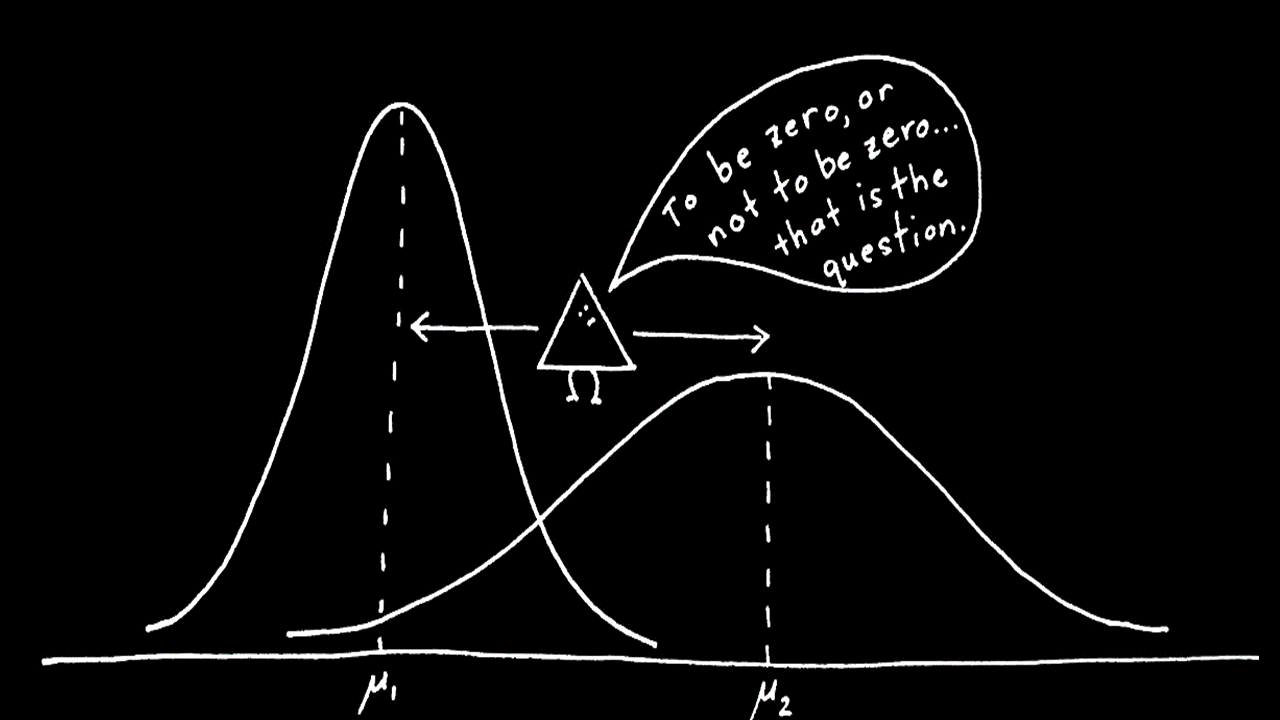
\includegraphics[scale=0.18]{TwoSample_Test-neg.png}\\
\end{center}
\pause
Multilevel designs:\\[1em]

\begin{enumerate}
\item Two methods applied to two independent sets of similar subjects.\\[1em]
E.g., comparing two products.
\vfill
\item Same method applied to two different kinds of subjects. \\[1em]
E.g., comparing bones of European kids and American kids.
\end{enumerate}
\end{frame}
%-------------- end slide -------------------------------%}}}
%-------------- start slide -------------------------------%{{{ 9.5
\begin{frame}{Test for normal parameters (two sample test)}
\begin{enumerate}
\item Let $X_1,\cdots, X_n$ be a random sample of size $n$ from $N(\mu_X,\sigma^2_X)$.	\\[1em]
\item Let $Y_1,\cdots, Y_m$ be a random sample of size $m$ from $N(\mu_Y,\sigma^2_Y)$.
\vfill
\item[Prob. 1] Find a test statistic $\Lambda$ in order to test\hfill $H_0 : \mu_X = \mu_Y$ v.s. $H_1 : \mu_X \ne \mu_Y$. \\[2em]
\item[1-1]When $\sigma^2_X$ and $\sigma^2_Y$ are known\\[1em]
\item[1-2]When $\sigma^2_X = \sigma^2_Y$ is unknown\\[1em]
\item[1-3]When $\sigma^2_X \ne \sigma^2_Y$, both are unknown
\pause \hspace{3em}
\vfill
\item[Prob. 2] Find a test statistic $\Lambda$ in order to test\hfill $H_0 : \sigma_X^2 = \sigma_Y^2$ v.s. $H_1 : \sigma_X^2 \ne \sigma^2_Y$. \\[2em]
\end{enumerate}
\end{frame}
%-------------- end slide -------------------------------%}}}
%-------------- start slide -------------------------------%{{{ 9.6
\begin{frame}
\begin{enumerate}
	\item[Prob. 1-1] Find a test statistic for $H_0 : \mu_X = \mu_Y$ v.s. $H_1 : \mu_X \ne \mu_Y$, \\[1em]
	with $\sigma^2_X$ and $\sigma^2_Y$ known.\\[2em]
	\vfill
	\item[Sol.]
	\[
		\frac{\overline{X}-\overline{Y}-(\mu_X-\mu_Y)}{\sqrt{\frac{\sigma_X^2}{n}+\frac{\sigma_Y^2}{m} }} =
		\frac{\overline{X}-\overline{Y}}{\sqrt{\frac{\sigma_X^2}{n}+\frac{\sigma_Y^2}{m} }} \sim N(0,1)
	\]
	\vfill
	\item[] Test statistics: $z = \frac{\bar{x}-\bar{y}}{\sqrt{\frac{\sigma_X^2}{n}+\frac{\sigma_Y^2}{m} }}$.
	\vfill
	\item[] Critical region $|z|\ge z_{\alpha/2}$. \myEnd
\end{enumerate}
\end{frame}
%-------------- end slide -------------------------------%}}}
%-------------- start slide -------------------------------%{{{ 9.7
\begin{frame}
\begin{enumerate}
	\item[Prob. 1-2] Find a test statistic for $H_0 : \mu_X = \mu_Y$ v.s. $H_1 : \mu_X \ne \mu_Y$, \\[1em]
		with $\sigma^2_X = \sigma^2_Y=\sigma^2$ but unknown.\\[2em]
\vfill
\item[Sol.] Composite-vs-composite test with:
\[\omega =\left\{(\mu_X,\mu_Y,\sigma^2): \mu_X=\mu_Y\in\R, \hspace{1.4em} \sigma^2>0\right\}\]
\[\Omega =\left\{(\mu_X,\mu_Y,\sigma^2): \mu_X\in\R,\: \mu_Y\in\R, \: \sigma^2>0\right\}\]\\[2em]
\item[] The likelihood function
	\begin{align*}
		L(\omega)= & \prod_{i=1}^n f_X(x_i) \prod_{j=1}^mf_Y(y_j)\\[2em]
		=&\left(  \frac{1}{\sqrt{2\pi}\:\sigma} \right)^{m+n}\exp \left(
	- \frac{1}{2\sigma^2} \left[\sum_{i=1}^n (x_i-\mu_X)^2 + \sum_{j=1}^m (y_i-\mu_Y)^2
	\right]
\right)
	\end{align*}
\end{enumerate}
\end{frame}
%-------------- end slide -------------------------------%}}}
%-------------- start slide -------------------------------%{{{ 9.8
\begin{frame}
	\begin{enumerate}
		\item[] Under $\omega$, the MLE $\omega_e=(\mu_{\omega_e},\mu_{\omega_e},\sigma_{\omega_e}^2)$ is\\[1em]
\begin{align*}
	\mu_{\omega_e} &=  \frac{\sum_{i=1}^n x_i+\sum_{j=1}^m y_j}{n+m}\\[2em]
	\sigma_{\omega_e}^2 &=   \frac{\sum_{i=1}^n (x_i-\mu_{\omega_e})^2+\sum_{j=1}^m (y_j-\mu_{\omega_e})^2}{n+m}
\end{align*}
\vfill
\item[] Hence,
	\[
		L(\omega_e) = \left(  \frac{e^{-1}}{2\pi\sigma_{\omega_e}^2}\right)^{ \frac{n+m}{2}}
	\]
	\end{enumerate}
\end{frame}
%-------------- end slide -------------------------------%}}}
%-------------- start slide -------------------------------%{{{ 9.9
\begin{frame}

	\begin{enumerate}
		\item[] Under $\Omega$, the MLE $\omega_e=(\mu_{X_e},\mu_{Y_e},\sigma_{\Omega_e}^2)$ is\\[1em]
			\[
				\mu_{X_e} =\frac{1}{n} \sum_{i=1}^{n}x_i \quad\text{and}\quad \mu_{Y_e}=\frac{1}{m} \sum_{j=1}^{m}y_j
			\]
			\\[1em]
			\[
				\sigma_{\Omega_e}^2 =
	 \frac{\sum_{i=1}^n (x_i-\mu_{X_e})^2+\sum_{j=1}^m (y_j-\mu_{Y_e})^2}{n+m}
			\]
			\vfill
		\item[] Hence,
			\[
				L(\Omega_e)
		= \left(  \frac{e^{-1}}{2\pi\sigma_{\Omega_e}^2}\right)^{ \frac{n+m}{2}}
			\]
	\end{enumerate}
\end{frame}
%-------------- end slide -------------------------------%}}}
%-------------- start slide -------------------------------%{{{ 9.10
\begin{frame}

	\begin{enumerate}
		\item[]
			\[
				\lambda =  \frac{L(\omega_e)}{L(\Omega_e)}= \left(  \frac{\sigma^2_{\Omega_e}}{\sigma^2_{\omega_e}}\right)^{ \frac{m+n}{2}}
			\]
			\vfill
\[
\lambda^{ \frac{2}{n+m}} =  \frac{\sum_{i=1}^n (x_i-\bar{x})^2+\sum_{j=1}^n (y_j-\bar{y})^2}{\sum_{i=1}^n \left(x_i- \frac{n\bar{x}+m\bar{y}}{m+n}\right)^2+\sum_{j=1}^n \left(y_j-\frac{n\bar{x}+m\bar{y}}{m+n}\right)^2}
\]
	\end{enumerate}
\end{frame}
%-------------- end slide -------------------------------%}}}
%-------------- start slide -------------------------------%{{{ 9.11
\begin{frame}
\begin{enumerate}
	\item []
		\begin{align*}
		\sum_{i=1}^n \left(x_i- \frac{n\bar{x}+m\bar{y}}{m+n}\right)^2 = \sum_{i=1}^n (x_i-\bar{x})^2 +  \frac{m^2n}{(m+n)^2} (\bar{x}-\bar{y})^2
		\end{align*}
		\vfill
		\begin{align*}
		\sum_{j=1}^m \left(y_j- \frac{n\bar{x}+m\bar{y}}{m+n}\right)^2 = \sum_{j=1}^m (y_i-\bar{y})^2 +  \frac{mn^2}{(m+n)^2} (\bar{x}-\bar{y})^2
	\end{align*}
		\vfill
	\item[]
		\begin{align*}
			\Downarrow
		\end{align*}
		\begin{gather*}
			\sum_{i=1}^n \left(x_i- \frac{n\bar{x}+m\bar{y}}{m+n}\right)^2+ \sum_{j=1}^n \left(y_j-\frac{n\bar{x}+m\bar{y}}{m+n}\right)^2 \\
				 || \\
			\sum_{i=1}^n (x_i-\bar{x})^2 + \sum_{j=1}^m (y_i-\bar{y})^2+  \frac{mn}{m+n} (\bar{x}-\bar{y})^2
		\end{gather*}
\end{enumerate}
\end{frame}
%-------------- end slide -------------------------------%}}}
%-------------- start slide -------------------------------%{{{ 9.12
\begin{frame}
	\begin{align*}
		\lambda^{ \frac{2}{m+n}} &=
		\frac{\sum_{i=1}^n (x_i-\bar{x})^2 + \sum_{j=1}^m (y_i-\bar{y})^2}{\sum_{i=1}^n (x_i-\bar{x})^2 + \sum_{j=1}^m (y_i-\bar{y})^2+  \frac{mn}{m+n}(\bar{x}-\bar{y})^2}\\[1em]
& =  \frac{1}{\displaystyle 1+  \frac{(\bar{x}-\bar{y})^2}{  \left[ \sum_{i=1}^n (x_i-\bar{x})^2 + \sum_{j=1}^m (y_i-\bar{y})^2 \right] \left( \frac{1}{m} + \frac{1}{n}  \right)}}
		\\[2em]& =  \frac{n+m-2}{\displaystyle n+m-2+  \frac{(\bar{x}-\bar{y})^2}{ \alert{ \frac{1}{n+m-2} \left[ \sum_{i=1}^n (x_i-\bar{x})^2 + \sum_{j=1}^m (y_i-\bar{y})^2 \right]} \left( \frac{1}{m} + \frac{1}{n}  \right)}}
		\\[2em] &=
		\frac{n+m-2}{\displaystyle n+m-2 +  \frac{(\bar{x}-\bar{y})^2}{\alert{s_p^2}\left(  \frac{1}{m}+  \frac{1}{n}\right)}}
		 =
		\frac{n+m-2}{n+m-2+t^2}.
	\end{align*}
	\vfill	\[
	\boxed{t :=  \frac{\bar{x}-\bar{y}}{s_p\sqrt{  \frac{1}{m}+  \frac{1}{n}} }}
	\]
\end{frame}
%-------------- end slide -------------------------------%}}}
%-------------- start slide -------------------------------%{{{ 9.13
\begin{frame}
\centering
\[
	t\mapsto  \frac{a}{a+t^2}
\]
\vfill
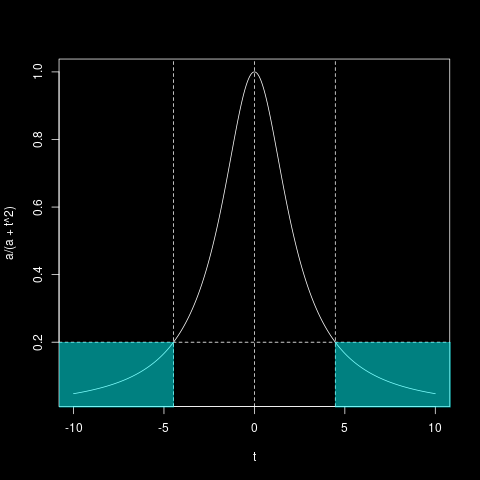
\includegraphics[scale=0.4]{T-Statistics-neg.png}
\end{frame}
%-------------- end slide -------------------------------%}}}
%-------------- start slide -------------------------------%{{{ 9.14
\begin{frame}

	\begin{enumerate}
		\item[] One can use the following statistic \\[1em]
			\[
				T =  \frac{\overline{X}-\overline{Y}}{S_p \sqrt{ \frac{1}{m}+ \frac{1}{n} }}
			\]
			\vfill
		\item[] where $S_p^2$ is called the \textcolor{yellow!80!black}{\it pooled sample variance}\\[1em]
			\begin{align*}
				S_p^2 =&  \frac{1}{n+m-2}\left[  \textcolor{magenta}{\sum_{i=1}^n \left(X_i -\overline{X} \right )^2}+ \textcolor{blue}{\sum_{i=1}^m \left(Y_j -\overline{Y} \right )^2}\right ]
				\\[1em] =&  \frac{1}{n+m-2}\left[ \textcolor{magenta}{(n-1)S_X^2} + \textcolor{blue}{(m-1) S_Y^2} \right ]
			\end{align*}
	\end{enumerate}
\end{frame}
%-------------- end slide -------------------------------%}}}
%-------------- start slide -------------------------------%{{{ 9.15
\begin{frame}
Three observations:
\vfill
	\begin{enumerate}
		\item $\E[\overline{X}-\overline{Y}] = 0$ and
			\[
\Var(\overline{X}-\overline{Y}) =
\Var(\overline{X})+ \Var(\overline{Y})
=  \frac{\sigma_X^2}{n} +  \frac{\sigma_Y^2}{m}
= \sigma^2 \left(  \frac{1}{n}+  \frac{1}{m}\right)
\]
\item[] Hence, $\textcolor{yellow}{\frac{\overline{X}-\overline{Y}}{\sigma\sqrt{\frac 1n + \frac 1m}}}\sim N(0,1)$
\vfill
\item $\textcolor{red}{\frac{n+m-2}{\sigma^2} S_p^2} = \sum_{i=1}^n \left(\frac{X_i-\overline{X}}{\sigma}\right)^2
	+ \sum_{j=1}^m \left(\frac{Y_j-\overline{Y}}{\sigma}\right)^2 \sim $ Chi square$(n+m-2)$
	\vfill
\item $\textcolor{yellow}{\frac{\overline{X}-\overline{Y}}{\sigma\sqrt{\frac 1n + \frac 1m}}} \perp  \textcolor{red}{\frac{n+m-2}{\sigma^2}S_p^2}$
	\vfill
\item[$\Longrightarrow$] $T = \frac{\displaystyle\textcolor{yellow}{\frac{\overline{X}-\overline{Y}}{\sigma\sqrt{\frac 1n+\frac 1m}}} }{\displaystyle\sqrt{\textcolor{red}{\frac{n+m-2}{\sigma^2} S_p^2}\times \frac{1}{n+m-2} }} = \frac{\overline{X}-\overline{Y}}{S_p \sqrt{ \frac{1}{m}+ \frac{1}{n} }} \sim $ t distr.$(n+m-2)$
	\end{enumerate}
\end{frame}
%-------------- end slide -------------------------------%}}}
%-------------- start slide -------------------------------%{{{ 9.16
\begin{frame}
	Finally, \\[2em]
\begin{enumerate}
	\item[] Test statistics: $t= \frac{\bar{x}-\bar{y}}{s_p\sqrt{\frac1m+\frac1n}}$
		\vfill
	\item[] Critical region: $|t|\ge t_{\alpha/2,n+m-2}$. \myEnd
\end{enumerate}
\end{frame}
%-------------- end slide -------------------------------%}}}
%-------------- start slide -------------------------------%{{{ 9.17
\begin{frame}
\begin{enumerate}
	\item[Prob. 1-3] Find a test statistic for $H_0 : \mu_X = \mu_Y$ v.s. $H_1 : \mu_X \ne \mu_Y$, \\[1em]
		with $\sigma^2_X \ne \sigma^2_Y$, both unknown.\\[2em]
		\vfill
	\item[Remark:] 1. Known as the {\it \textcolor{yellow}{Behrens-Fisher problem}}.
			\vfill
		\item[] 2. No exact solutions!
			\vfill
		\item[] 3. We will derive a widely used approximation by
			\vspace{3em}
			% \\[2em]
		\item[]	\hspace{5em} {\it Bernard Lewis Welch} (1911--1989)
\end{enumerate}

\end{frame}
%-------------- end slide -------------------------------%}}}
%-------------- start slide -------------------------------%{{{ 9.18
\begin{frame}

	\begin{enumerate}
		\item[Sol.]
	\[
W =  \frac{\overline{X}-\overline{Y}-(\mu_X-\mu_Y)}{\sqrt{ \frac{S^2_X}{n}+\frac{S^2_Y}{m}  }}
=  \frac{\overline{X}-\overline{Y}-(\mu_X-\mu_Y)}{\sqrt{ \frac{\sigma^2_X}{n}+\frac{\sigma^2_Y}{m}  }}
\Bigg/  \frac{\sqrt{ \frac{S^2_X}{n}+\frac{S^2_Y}{m}  }}{\sqrt{ \frac{\sigma^2_X}{n}+\frac{\sigma^2_Y}{ m} }}
\]
\vfill \item[]
\[
U:=\frac{\overline{X}-\overline{Y}-(\mu_X-\mu_Y)}{\sqrt{ \frac{\sigma^2_X}{n}+\frac{\sigma^2_Y}{m} }}\sim N(0,1)
\]
\vfill
\item[]
\[
\frac{V}{\nu}:= \frac{\displaystyle\frac{S^2_X}{n}+\frac{S^2_Y}{m}}{\displaystyle\frac{\sigma^2_X}{n}+\frac{\sigma^2_Y}{m}}
\]
	\end{enumerate}
\end{frame}
%-------------- end slide -------------------------------%}}}
%-------------- start slide -------------------------------%{{{ 9.19
\begin{frame}
\begin{itemize}
	\item[!!] {\bf Assumption/Approximation:} \\[1em]
		Assume that $V$ follows Chi Square$(\nu)$ and assume that $V\perp U$.
	\vfill
\item[$\Longrightarrow$] Then, $W\sim$ Student's t-distribution of freedom $\nu$.
	\vfill
\item[?] It remains to estimate $\nu$: Suppose we have
\[
\nu= \frac{\left(  \frac{\sigma_X^2}{n}+ \frac{\sigma_Y^2}{m} \right)^2 }
{ \frac{\sigma_X^4}{n^2(n-1)}+\frac{\sigma_Y^4}{m^2(m-1) }}
=
\frac{\left(\theta+ \frac{n}{m} \right)^2}{ \frac{1}{n-1}\theta^2 +  \frac{1}{m-1}\left(  \frac{n}{m}\right)^2},
\quad \theta= \frac{\sigma_X^2}{\sigma_Y^2}.
\]
\vfill
\item[!!] Still need to know $\theta = \sigma_X^2/\sigma_Y^2$... Another approximation $\hat\theta=S_X^2/S_Y^2$, i.e., \\[1em]
\[
\nu \approx
\frac{\left(\frac{s_X^2}{n}+ \frac{s_Y^2}{m} \right)^2 }
{ \frac{s_X^4}{n^2(n-1)}+\frac{s_Y^4}{m^2(m-1) }}
=  \frac{\left(\hat\theta+ \frac{n}{m} \right)^2}{ \frac{1}{n-1}\hat\theta^2 +  \frac{1}{m-1}\left(  \frac{n}{m}\right)^2},
\quad \hat\theta= \frac{s_X^2}{s_Y^2}.
\]
\end{itemize}

\end{frame}
%-------------- end slide -------------------------------%}}}
%-------------- start slide -------------------------------%{{{ 9.20
\begin{frame}

\begin{enumerate}
	\item[] In summary: \\[1em]
		\[
			W =  \frac{\overline{X}-\overline{Y}-(\mu_X-\mu_Y)}{\sqrt{ \frac{S^2_X}{n}+\frac{S^2_Y}{m} }}
			\sim \text{Student's t of freedom $\nu$}
		\]
\vfill
\item[]
\[
	\nu  = \left[
\frac{\left(\frac{s_X^2}{n}+ \frac{s_Y^2}{m} \right)^2 }
{ \frac{s_X^4}{n^2(n-1)}+\frac{s_Y^4}{m^2(m-1) }}
	\right]
	=
	\left[
\frac{\left(\hat\theta+ \frac{n}{m} \right)^2}{ \frac{1}{n-1}\hat\theta^2 +  \frac{1}{m-1}\left(  \frac{n}{m}\right)^2}
	\right],
\quad \hat\theta= \frac{s_X^2}{s_Y^2}.
\]
\vfill
\item[] Test statistic: $t = \frac{\bar{x}-\bar{y}-(\mu_X-\mu_Y)}{\sqrt{ \frac{s^2_X}{n}+\frac{s^2_Y}{m} }}
$
\vfill
\item[] Critical region: $|t|\ge t_{\alpha/2,\nu}$.\myEnd
	\vfill
\item[Remark] If $\nu \ge 100$, replace the t-score, e.g., $t_{\alpha/2,\nu}$ by the z-score, e.g., $z_{\alpha/2}$.
	\end{enumerate}
\end{frame}
%-------------- end slide -------------------------------%}}}
%-------------- start slide -------------------------------%{{{ 9.21
\begin{frame}

	\begin{enumerate}
		\item[Thm ] The moment estimate for $\nu$
			\begin{align*}
	\nu &=   \frac{\left(  \frac{\sigma_X^2}{n}+ \frac{\sigma_Y^2}{m} \right)^2 }
{ \frac{\sigma_X^4}{n^2(n-1)}+\frac{\sigma_Y^4}{m^2(m-1) }+ \frac{\sigma_X^2\sigma_Y^2}{mn}}
	\\[2em] & \approx
\frac{\left(  \frac{\sigma_X^2}{n}+ \frac{\sigma_Y^2}{m} \right)^2 }
{ \frac{\sigma_X^4}{n^2(n-1)}+\frac{\sigma_Y^4}{m^2(m-1) }}
=
\frac{\left(\theta+ \frac{n}{m} \right)^2}{ \frac{1}{n-1}\theta^2 +  \frac{1}{m-1}\left(  \frac{n}{m}\right)^2},
\quad \theta= \frac{\sigma_X^2}{\sigma_Y^2}.
			\end{align*}
\vfill
\item[Proof.]
\[
	\frac{V}{\nu}\left( \frac{\sigma^2_X}{n}+\frac{\sigma^2_Y}{m} \right)= \frac{S^2_X}{n}+\frac{S^2_Y}{m}
\]
\vfill
\item[]$(n-1)S_X^2/\sigma_X^2\sim$ Chi Sqr$(n-1) \Longrightarrow\E(S_X^2)= \sigma_X^2$. Similarly, $\E(S_Y^2)= \sigma_Y^2$.
	\end{enumerate}
\end{frame}
%-------------- end slide -------------------------------%}}}
%-------------- start slide -------------------------------%{{{ 9.22
\begin{frame}

	\begin{enumerate}
\item[] First moment gives identity. Need to consider second moment.
\item[] Second moments for Chi sqr(r) is $2r$. Hence, $\E(S_X^4) =  \frac{\sigma_X^4}{n-1}$.
\item[]
			\begin{align*}
			 \frac{2\nu}{\nu^2}
	\left( \frac{\sigma^2_X}{n}+\frac{\sigma^2_Y}{m} \right)^2
	&= 2\frac{\sigma^4_X}{n^2(n-1)}+2\frac{\sigma^4_Y}{m^2(m-1)}
	+  2\frac{\sigma_X^2\sigma_Y^2}{mn}
				% \\[2em]&\approx 2\frac{\sigma^4_X}{n^2(n-1)}+2\frac{\sigma^4_Y}{m^2(m-1)}
			\end{align*}
		\item[] ... \myEnd
			\vfill
	\item[Remark] Welch (1938) approximation is more involved, which actually assumes that $V$ follows the {\it Type III Pearson distribution}.
	\item[]	\url{https://en.wikipedia.org/wiki/Behrens-Fisher_problem}
	\end{enumerate}
\end{frame}
%-------------- end slide -------------------------------%}}}
%-------------- start slide -------------------------------%{{{ 9.23
\begin{frame}
	\begin{enumerate}
		\item[Prob. 2] Find a test statistic $\Lambda$ in order to test\qquad $H_0 : \sigma_X^2 = \sigma_Y^2$ v.s. $H_1 : \sigma_X^2 \ne \sigma^2_Y$. \\[2em]
		\vfill
		\item[Sol.]
			\[
			\frac{S_X^2/\sigma_X^2}{S_Y^2/\sigma_Y^2} \sim \text{F-disribution $(n-1,m-1)$}
			\]
			\vfill
		\item[] Test statistic: $f =\frac{s_X^2/\sigma_X^2}{s_Y^2/\sigma_Y^2}=\frac{s_X^2}{s_Y^2} $
			\vfill
		\item[] Critical regions: $f\le  F_{\alpha/2,n-1,m-1}$ or $f\ge F_{1-\alpha/2,n-1,m-1}$. \myEnd
	\end{enumerate}
\end{frame}
%-------------- end slide -------------------------------%}}}

\mySection{9.2 Testing $H_0:\mu_X=\mu_Y$}
%-------------- start slide -------------------------------%{{{ 9.26
\begin{frame}
	% {\S\: 9.2 Testing $H_0:\mu_X=\mu_Y$}
\begin{itemize}
	\item Let $X_1,\cdots, X_n$ be a random sample of size $n$ from $N(\mu_X,\sigma^2_X)$.	\\[1em]
	\item Let $Y_1,\cdots, Y_m$ be a random sample of size $m$ from $N(\mu_Y,\sigma^2_Y)$.
\end{itemize}
\vfill
\begin{center}
\begin{minipage}{0.5\textwidth}
\begin{enumerate}
	\item[Prob. 1] Testing $H_0:\mu_X=\mu_Y$ if $\sigma_X^2 = \sigma_Y^2$. \\[3em]
	\item[Prob. 2] Testing $H_0:\mu_X=\mu_Y$ if $\sigma_X^2 \ne \sigma_Y^2$.
\end{enumerate}
\end{minipage}
\end{center}
\vfill
\mySeparateLine
\vfill

\begin{minipage}{0.4\textwidth}
	\begin{itemize}
		\item True means: \hfill $\mu_X$, $\mu_Y$
		\item True std. dev.'s: \hfill $\sigma_X$, $\sigma_Y$
		\item True variances:\hfill  $\sigma_X^2$, $\sigma_Y^2$\\[2em]
		% \item Sample means:\hfill  $\overline{X}$, $\overline{Y}$
		% \item Sample std. dev.'s: \hfill $S_X$, $S_Y$
		% \item Sample variances: \hfill $S_X^2$, $S_Y^2$
	\end{itemize}
\end{minipage}
\hfill
\begin{minipage}{0.45\textwidth}
	\begin{itemize}
		% \item True means: \hfill $\mu_X$, $\mu_Y$
		% \item True std. dev.'s: \hfill $\sigma_X$, $\sigma_Y$
		% \item True variances:\hfill  $\sigma_X^2$, $\sigma_Y^2$\\[2em]
		\item Sample means:\hfill  $\overline{X}$, $\overline{Y}$
		\item Sample std. dev.'s: \hfill $S_X$, $S_Y$
		\item Sample variances: \hfill $S_X^2$, $S_Y^2$
	\end{itemize}
\end{minipage}
\end{frame}
%-------------- end slide -------------------------------%}}}
%-------------- start slide -------------------------------%{{{ 9.27
\begin{frame}{When $\sigma_X^2=\sigma_Y^2 = \sigma^2$}
\begin{itemize}
	\item[Def.] The \textcolor{yellow!80!black}{\bf pooled variance}:
		$\displaystyle S_p^2 =\frac{(n-1)S_X^2+(m-1)S_Y^2}{n+m-2}$\\[2em]
	\hspace{11.5em} $\displaystyle
	= \frac{\sum_{i=1}^n (X_i-\overline{X})^2+ \sum_{j=1}^n (Y_j-\overline{Y})^2 }{n+m-2}$
\vfill
\item[Thm.]
$\displaystyle T_{n+m-2}=\frac{\overline{X}-\overline{Y}-(\mu_X-\mu_Y)}{S_p\sqrt{ \frac{1}{n}+\frac{1}{m} }}$
$\sim$
Student t distr. of $n+m-2$ dgs of fd.
\vfill
\item[Proof.] (See slides on Section 9.1) \myEnd
\end{itemize}
\end{frame}
%-------------- end slide -------------------------------%}}}
%-------------- start slide -------------------------------%{{{ 9.28
\begin{frame}{When $\sigma_X^2=\sigma_Y^2 = \sigma^2$}

\centering
Testing $H_0:\mu_X = \mu_Y$ v.s.\\[1em]
(at the $\alpha$ level of significance)
\\[1em]
$\displaystyle t=\frac{\bar{x}-\bar{y}}{s_p\sqrt{ \frac{1}{n}+\frac{1}{m} }}$
\vfill

\begin{minipage}{0.32\textwidth}
\centering
$H_1:\mu_X <\mu_Y$:\\[1em]
Reject $H_0$ if \\[1em]
$t \le -t_{\alpha,n+m-2}$
\end{minipage}
\begin{minipage}{0.32\textwidth}
\centering
$H_1:\mu_X \ne \mu_Y$:\\[1em]
Reject $H_0$ if \\[1em]
$|t| \ge t_{\alpha/2,n+m-2}$
\end{minipage}
\begin{minipage}{0.32\textwidth}
\centering
$H_1:\mu_X>\mu_Y$:\\[1em]
Reject $H_0$ if \\[1em]
$t \ge t_{\alpha,n+m-2}$
\end{minipage}
\end{frame}
%-------------- end slide -------------------------------%}}}
%-------------- start slide -------------------------------%{{{ 9.29
\begin{frame}
\begin{itemize}
\item[E.g.] Test whether Mark Twain and Snodgrass are the same person by checking the proportion of three-letter words at the $99\%$ level of significance.
\begin{center}
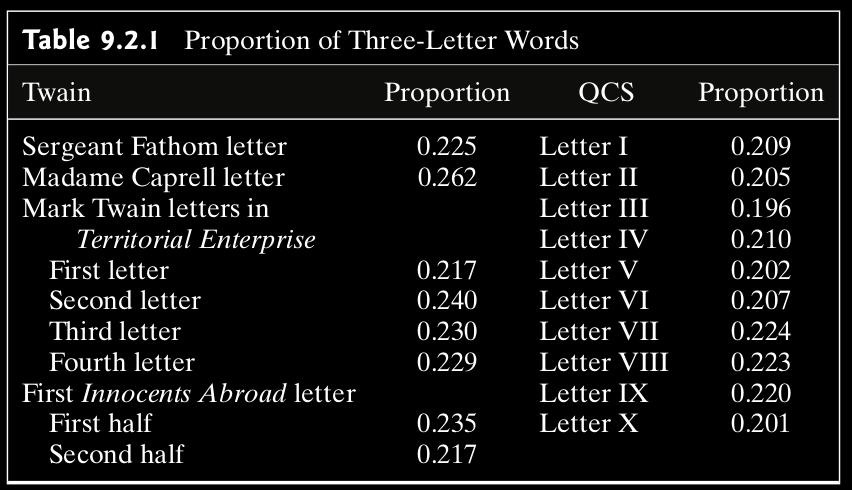
\includegraphics[scale=0.2]{Table_9-2-1-neg.png}
\end{center}
\vfill
\item[Sol.] We need to test
	\[
	H_0: \mu_X = \mu_Y \quad v.s. \quad H_1: \mu_X\ne \mu_Y.
	\]
	Since we are tesing whether they are the same person, one can assume that $\sigma_X^2 = \sigma_Y^2$.
\end{itemize}
\end{frame}
%-------------- end slide -------------------------------%}}}
%-------------- start slide -------------------------------%{{{ 9.30
\begin{frame}
\begin{enumerate}
\item $n=8$, $m=10$,
\begin{align*}
&\sum_{i=1}^n x_i = 1.855,\quad \sum_{i=1}^n x_i^2 = 0.4316\\
&\sum_{i=1}^m y_i = 2.097,\quad \sum_{i=1}^m y_i^2 = 0.4406
\end{align*}
\vfill
\item Hence,
	\[
		\bar{x} = 1.855/8=02319 \quad \bar{y}=2.097/10 =0.2097
	\]
	\[
		s_X^2 =  \frac{8\times 0.4316-1.855^2}{8\times 7}=0.0002103
	\]
	\[
		s_Y^2 =  \frac{10\times 0.4406-2.097^2}{10\times 9}=0.0000955
	\]
	\[
		s_p^2 =  \frac{(n-1)s_X^2+(m-1)s_Y^2}{n+m-2} =...=0.0001457
	\]
	\[
		t=  \frac{\bar{x}-\bar{y}}{s_p\sqrt{ \frac{1}{n}+ \frac{1}{m} }} = ... = 3.88
	\]
\end{enumerate}
\end{frame}
%-------------- end slide -------------------------------%}}}
%-------------- start slide -------------------------------%{{{ 9.31
\begin{frame}
	\begin{itemize}
		\item[3.] Critical region: $|t|\ge t_{0.005,n+m-2} = t_{0.005,16} = 2.9208$. \\[1em]
			\begin{center}
				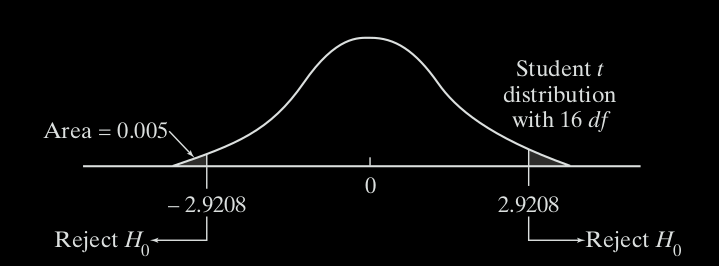
\includegraphics[scale=0.3]{Figure_9-2-1-neg.png}
			\end{center}
		 \vfill
		\item[4.] Conclusion: Rejection! \myEnd
	\end{itemize}
\end{frame}
%-------------- end slide -------------------------------%}}}
%-------------- start slide -------------------------------%{{{ 9.32
\begin{frame}

	\begin{enumerate}
		\item[E.g.] Comparing large-scales and small-scales companies:\\[1em]
			Based on the data below, can we say that the return o equity differs between the two types of companies?
			\vfill
			\begin{center}
			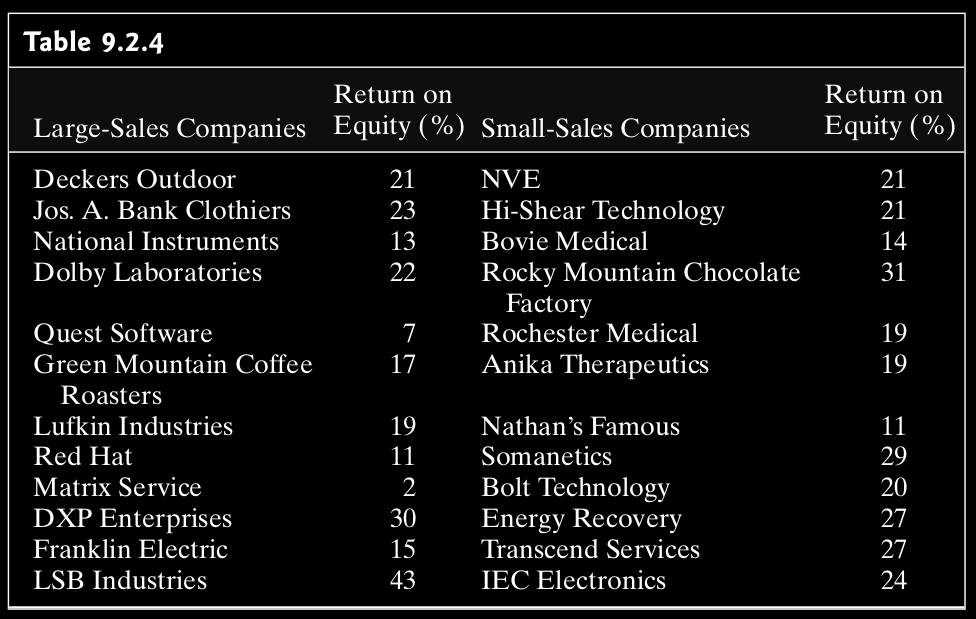
\includegraphics[scale=0.2]{Table_9-2-4-neg.png}
			\end{center}
	\end{enumerate}
\end{frame}
%-------------- end slide -------------------------------%}}}
%-------------- start slide -------------------------------%{{{ 9.33
\begin{frame}
	\begin{enumerate}
		\item[Sol.] Let $\mu_X$ and $\mu_Y$ be the average returns. We are asked to test\\[1em]
			\[
			H_0: \mu_X = \mu_Y \qquad v.s. \qquad H_1: \mu_X\ne \mu_Y.
			\]
			\vfill
		\item[1.]
			\[
			n=12,\qquad	\sum_{i=1}^n x_i = 223
				\qquad
				\sum_{i=1}^n x_i^2 = 5421
			\]
			\[
			m=12,\qquad	\sum_{i=1}^m y_i = 263
				\qquad
				\sum_{i=1}^m y_i^2 = 6157
			\]
		\item[2.]
			\[
				\bar{x} = 18.5833,\qquad s_X^2 = 116.0833
			\]
			\[
				\bar{y} = 21.9167, \qquad s_Y^2 = 35.7197
			\]
			\[
				w= \frac{18.5833 -21.9167 }{\sqrt{ \frac{116.0833}{12}+  \frac{35.7197}{12} }} = -0.9371932.
			\]
			\[
				\hat\theta =  \frac{116.0833}{35.7179} = 3.250 \quad\Rightarrow\quad
				\nu = \left[ \frac{(3.250+1)^2}{ \frac{1}{11}3.250^2+ \frac{1}{11} 1^2 } \right]
				=\left[ 17.18403\right] = 17.
			\]
	\end{enumerate}
\end{frame}
%-------------- end slide -------------------------------%}}}
%-------------- start slide -------------------------------%{{{ 9.34
\begin{frame}
	\begin{itemize}
		\item[3.] The critical region is $|w|\ge t_{\alpha/2,17} = 2.1098$.\\[2em]
		\item[4.] Conclusion: \\[1em] Since $w= -0.94$ is not in the critical region, we fail to reject $H_0$. \myEnd
	\end{itemize}
\end{frame}
%-------------- end slide -------------------------------%}}}

\mySection{9.3 Testing $H_0:\sigma_X^2=\sigma_Y^2$}
%-------------- start slide -------------------------------%{{{ 9.37
\begin{frame}
	% {\S\: 9.3 Testing $H_0:\sigma_X^2=\sigma_Y^2$}
\begin{enumerate}
	\item[Mot. 1]
	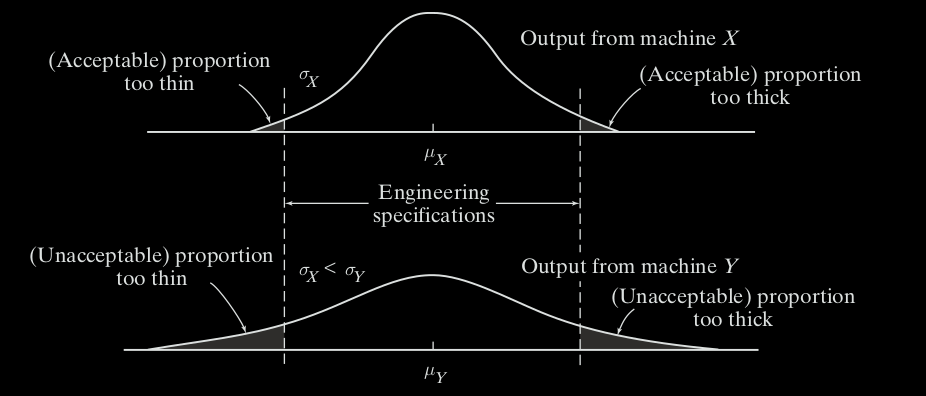
\includegraphics[scale=0.35]{Figure_9-3-1-neg.png}
	\vfill
\item[Mot. 2] To test $H_0:\mu_X=\mu_Y$ under the assumption $\sigma_X^2=\sigma_Y^2$, we need to first test $\sigma_X^2 = \sigma_Y^2$.
	\end{enumerate}
\end{frame}
%-------------- end slide -------------------------------%}}}
%-------------- start slide -------------------------------%{{{ 9.38
\begin{frame}
\centering
Testing $H_0:\sigma_X^2 = \sigma_Y^2$ \\[1em]
v.s.\\[1em]
(at the $\alpha$ level of significance)
\\
\vfill

\begin{minipage}{0.32\textwidth}
\centering
$H_1:\sigma_X^2 <\sigma_Y^2$:\\[1em]
Reject $H_0$ if \\[1em]
$s_Y^2/s_X^2\le F_{\alpha,m-1,n-1}$\\
\vspace{1.2em}
\phantom{aaa}
\end{minipage}
\begin{minipage}{0.32\textwidth}
\centering
$H_1:\sigma^2_X \ne \sigma^2_Y$:\\[1em]
Reject $H_0$ if \\[1em]
$s_Y^2/s_X^2 \ge F_{1-\alpha/2,m-1,n-1}$ or\\
$s_Y^2/s_X^2 \le F_{\alpha/2,m-1,n-1}$
\end{minipage}
\begin{minipage}{0.32\textwidth}
\centering
$H_1:\sigma^2_X>\sigma^2_Y$:\\[1em]
Reject $H_0$ if \\[1em]
$s_Y^2/s_X^2\ge F_{1-\alpha,m-1,n-1}$\\
\vspace{1.2em}
\phantom{aaa}
\end{minipage}
\end{frame}
%-------------- end slide -------------------------------%}}}
%-------------- start slide -------------------------------%{{{ 9.39
\begin{frame}
\begin{itemize}
	\item[E.g.] Electroencephalograms (EEG). \\[1em]
		Twenty inmates in a Canadian prison, randomly split into
		two groups of equal size: one in solitary confinement, one in their own cells.\\[1em]
		Measure the alpha waves.
		Whether the observed difference in variability is significant (set $\alpha=0.05$.)\\
		\vfill
		\begin{minipage}{0.45\textwidth}
			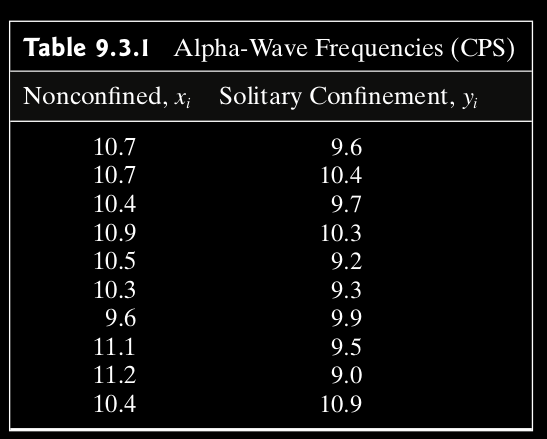
\includegraphics[scale=0.2]{Table_9-3-1-neg.png}
\end{minipage}
		\begin{minipage}{0.45\textwidth}
			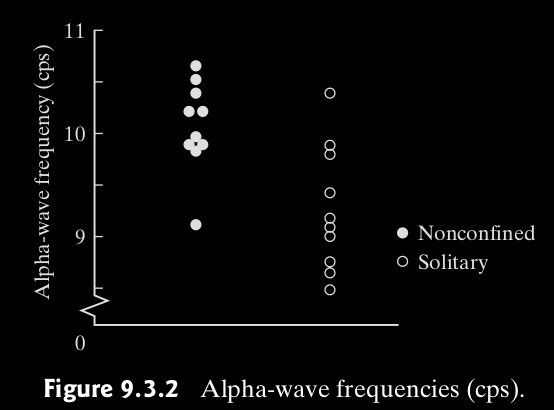
\includegraphics[scale=0.2]{Figure_9-3-2-neg.png}
\end{minipage}
\vfill
\item[Sol.] ... \myEnd
\end{itemize}
\end{frame}
%-------------- end slide -------------------------------%}}}
%-------------- start slide -------------------------------%{{{ 9.40
\begin{frame}
Another example here: \\[2em]
\url{https://www.itl.nist.gov/div898/handbook/eda/section3/eda359.htm}
\end{frame}
%-------------- end slide -------------------------------%}}}

\mySection{9.4 Binomial Data: Testing $H_0:p_X=p_Y$}
%-------------- start slide -------------------------------%{{{ 9.43
\begin{frame}
		% {\S\: 9.4 Binomial Data: Testing $H_0:p_X=p_Y$}
By the central limit theorem, when $n$ and $m$ are large\\[1em]
\[
\frac{ \frac{X}{n}-  \frac{Y}{m}-\E\left(  \frac{X}{n}- \frac{Y}{m}\right)}{\sqrt{\Var\left(  \frac{X}{n}- \frac{Y}{m}\right)}} \stackrel{approx.}{\sim} N(0,1)
\]
\vfill \pause
Under $H_0: p_X=p_Y$, \\[1em]
\[
\E\left(  \frac{X}{n}-  \frac{Y}{m}\right) = 0
\]
\\[1em]\pause
\[
\Var\left(  \frac{X}{n}- \frac{Y}{m}\right) =  \frac{p(1-p)}{n}+\frac{p(1-p)}{m}
\]
\vfill\pause
The MLE for $p$ under $H_0$ is\\[1em]
\[
p_e= \frac{x+y}{n+m}
\]
\end{frame}
%-------------- end slide -------------------------------%}}}
%-------------- start slide -------------------------------%{{{ 9.44
\begin{frame}
\centering
Testing $H_0:p_X = p_Y$ \\[1em]
v.s.\\[1em]
(at the $\alpha$ level of significance)\\[1em]
\[
z= \frac{ \frac{x}{n}-\frac{y}{m}}{\sqrt{ p_e(1-p_e) \left( \frac{1}{n}+ \frac{1}{m} \right)}}
,\qquad p_e= \frac{x+y}{n+m}
\]
\\
\vfill

\begin{minipage}{0.32\textwidth}
\centering
$H_1:p_X <p_Y$:\\[1em]
Reject $H_0$ if \\[1em]
$z\le -z_{\alpha}$
\end{minipage}
\begin{minipage}{0.32\textwidth}
\centering
$H_1:p_X \ne p_Y$:\\[1em]
Reject $H_0$ if \\[1em]
$|z| \ge z_{\alpha/2}$
\end{minipage}
\begin{minipage}{0.32\textwidth}
\centering
$H_1:p_X>p_Y$:\\[1em]
Reject $H_0$ if \\[1em]
$z\ge z_{\alpha}$
\end{minipage}
\end{frame}
%-------------- end slide -------------------------------%}}}
%-------------- start slide -------------------------------%{{{ 9.45
\begin{frame}

\begin{enumerate}
\item[E.g.] Nightmares among men and women:
\begin{center}
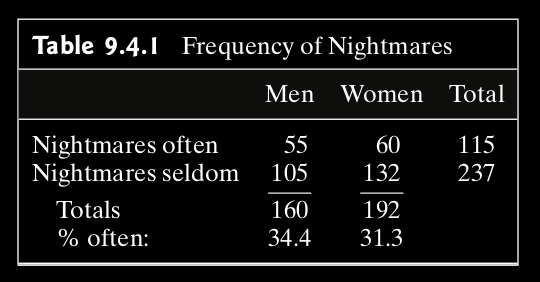
\includegraphics[scale=0.25]{Table_9-4-1-neg.png}
\end{center}
Is 34.4\% significantly different from 31.1\% ($\alpha=0.05$)?
\vfill
\item[Sol.] ... \myEnd
\end{enumerate}
\end{frame}
%-------------- end slide -------------------------------%}}}

\mySection{9.5  Confidence Intervals for the Two-Sample Problem}
%-------------- start slide -------------------------------%{{{ 9.48
\begin{frame}
	% {\S\: 9.5 Confidence Intervals for the Two-Sample Problem}
	\centering
	Similar to the hypothesis test ...
\end{frame}
%-------------- end slide -------------------------------%}}}
%-------------- start slide -------------------------------%{{{ 9.49
\begin{frame}
\begin{enumerate}
\item Let $X_1,\cdots, X_n$ be a random sample of size $n$ from $N(\mu_X,\sigma^2_X)$.	\\[1em]
\item Let $Y_1,\cdots, Y_m$ be a random sample of size $m$ from $N(\mu_Y,\sigma^2_Y)$.
\vfill
\item[Prob. 1] Find the $100(1-\alpha)\%$ C.I. for $\mu_X-\mu_Y$\\[2em]
\item[]When both $\sigma^2_X$ and $\sigma^2_Y$ are known\\[1em]
\item[]When $\sigma^2_X = \sigma^2_Y=\sigma^2$, but is unknown\\[1em]
\item[]When $\sigma^2_X \ne \sigma^2_Y$, both are unknown
\pause \hspace{3em}
\vfill
\item[Prob. 2] Find the $100(1-\alpha)\%$ C.I. for $\sigma_X^2/\sigma_Y^2$, or $\sigma_X/\sigma_Y$\\[2em]
\end{enumerate}
\end{frame}
%-------------- end slide -------------------------------%}}}
%-------------- start slide -------------------------------%{{{ 9.50
\begin{frame}
\begin{enumerate}
\item[Prob. 1-1] Find the $100(1-\alpha)\%$ C.I. for $\mu_X-\mu_Y$ with $\sigma^2_X$ and $\sigma^2_Y$ known.
	\vfill
\item[Sol.]
	\[
		\frac{\overline{X}-\overline{Y} - (\mu_X-\mu_Y)}{\sqrt{\frac{\sigma_X^2}{n} + \frac{\sigma_Y^2}{m} }}\sim N(0,1)
	\]
	\vfill
\item[]
	\[
		\bbP \left(-z_{\alpha/2} \le \frac{\overline{X}-\overline{Y} - (\mu_X-\mu_Y)}{\sqrt{\frac{\sigma_X^2}{n} + \frac{\sigma_Y^2}{m} }}\le z_{\alpha/2}\right )=1-\alpha
	\]
	\[||\]
	\[
		\hspace{-3.5em}	\bbP \left(
			(\overline{X}-\overline{Y})-z_{\alpha/2} \sqrt{\frac{\sigma_X^2}{n} + \frac{\sigma_Y^2}{m}}
			\le  \mu_X-\mu_Y \le
			(\overline{X}-\overline{Y})+z_{\alpha/2} \sqrt{\frac{\sigma_X^2}{n} + \frac{\sigma_Y^2}{m}}
		\right )
	\]
	\vfill
\item[]
	\[
		\left(
			(\overline{x}-\overline{y})-z_{\alpha/2} \sqrt{\frac{\sigma_X^2}{n} + \frac{\sigma_Y^2}{m}}
\quad,\quad
(\overline{x}-\overline{y})+z_{\alpha/2} \sqrt{\frac{\sigma_X^2}{n} + \frac{\sigma_Y^2}{m}}
\right )
	\]
	\myEnd
\end{enumerate}
\end{frame}
%-------------- end slide -------------------------------%}}}
%-------------- start slide -------------------------------%{{{ 9.51
\begin{frame}
\begin{enumerate}
\item[Prob. 1-2] Find the $100(1-\alpha)\%$ C.I. for $\mu_X-\mu_Y$ when $\sigma^2_X = \sigma^2_Y=\sigma^2$ unknown
	\vfill
\item[Sol.]
	\[
		\frac{\overline{X}-\overline{Y} - (\mu_X-\mu_Y)}{S_p\sqrt{\frac 1n + \frac 1m}}\sim \text{Student t-distribution $(n+m-2)$}
	\]
	\vfill
\item[]
	\[
		\bbP \left(-t_{\alpha/2,n+m-2} \le \frac{\overline{X}-\overline{Y} - (\mu_X-\mu_Y)}{S_p\sqrt{\frac 1n + \frac 1m}}\le t_{\alpha/2,n+m-2}\right ) = 1-\alpha
	\]
	\[||\]
	\[
		\hspace{-3.5em}	\bbP \left(
			(\overline{X}-\overline{Y})-t_{\alpha/2,n+m-2} S_p\sqrt{\frac 1n + \frac 1m}
			\le  \mu_X-\mu_Y \le
			(\overline{X}-\overline{Y})+t_{\alpha/2,n+m-2} S_p\sqrt{\frac 1n + \frac 1m}
		\right )
	\]
	\vfill
\item[]
	\[
		\left(
(\overline{x}-\overline{y})-t_{\alpha/2,n+m-2} s_p\sqrt{\frac 1n + \frac 1m}
\quad,\quad
(\overline{x}-\overline{y})+t_{\alpha/2,n+m-2} s_p\sqrt{\frac 1n + \frac 1m}
\right )
	\]
	\myEnd
\end{enumerate}
\end{frame}
%-------------- end slide -------------------------------%}}}
%-------------- start slide -------------------------------%{{{ 9.52
\begin{frame}
\begin{enumerate}
\item[Prob. 1-3] Find the $100(1-\alpha)\%$ C.I. for $\mu_X-\mu_Y$ when $\sigma^2_X \ne \sigma^2_Y$ unknown.
	\vfill
\item[Sol.]
	\[
		\frac{\overline{X}-\overline{Y} - (\mu_X-\mu_Y)}{\sqrt{\frac{S_X^2}{n} + \frac{S_Y^2}{m} }}\sim \text{Student t-distribution $(\nu)$}
	\]
	\vfill
\item[]
	\[
		\bbP \left(-t_{\alpha/2,\nu} \le \frac{\overline{X}-\overline{Y} - (\mu_X-\mu_Y)}{\sqrt{\frac{S_X^2}{n} + \frac{S_Y^2}{m} }}\le t_{\alpha/2,\nu}\right ) \approx 1-\alpha
	\]
	\[||\]
	\[
		\hspace{-3.5em}	\bbP \left(
			(\overline{X}-\overline{Y})-t_{\alpha/2,\nu} \sqrt{\frac{S_X^2}{n} + \frac{S_Y^2}{m}}
			\le  \mu_X-\mu_Y \le
			(\overline{X}-\overline{Y})+t_{\alpha/2,\nu} \sqrt{\frac{S_X^2}{n} + \frac{S_Y^2}{m}}
		\right )
	\]
	\vfill
\item[]
	\[
		\left(
			(\overline{x}-\overline{y})-t_{\alpha/2,\nu} \sqrt{\frac{s_X^2}{n} + \frac{s_Y^2}{m}}
\quad,\quad
(\overline{x}-\overline{y})+t_{\alpha/2,\nu} \sqrt{\frac{s_X^2}{n} + \frac{s_Y^2}{m}}
\right )
	\]
	\myEnd
\end{enumerate}
\end{frame}
%-------------- end slide -------------------------------%}}}
%-------------- start slide -------------------------------%{{{ 9.53
\begin{frame}
	\begin{enumerate}
\item[Prob. 2] Find the $100(1-\alpha)\%$ C.I. for $\sigma_X^2/\sigma_Y^2$
	\vfill
\item[Sol 1.]
	\[
		\frac{S_X^2/\sigma_X^2}{S_Y^2/\sigma_Y^2} \sim \text{F-disribution $(n-1,m-1)$}
	\]
		\[
		\bbP \left(F_{\alpha/2,n-1,m-1} \le\frac{S_X^2/\sigma_X^2}{S_Y^2/\sigma_Y^2}
	\le F_{1-\alpha/2,n-1,m-1}\right) =1-\alpha
	\]
	\[||\]
	\[
		\hspace{-3.5em}	\bbP \left(
			\frac{S_X^2}{S_Y^2}  \frac{1}{F_{1-\alpha/2,n-1,m-1}}
			\le
\frac{\sigma_X^2}{\sigma_Y^2}
\le
			\frac{S_X^2}{S_Y^2}  \frac{1}{F_{\alpha/2,n-1,m-1}}
		\right )
	\]
\item[]
	\vfill
	\[
		\left(
			\frac{s_X^2}{s_Y^2}  \frac{1}{F_{1-\alpha/2,n-1,m-1}}
			\quad,\quad
			\frac{s_X^2}{s_Y^2}  \frac{1}{F_{\alpha/2,n-1,m-1}}
		 \right )
	\]
\myEnd
	\end{enumerate}
\end{frame}
%-------------- end slide -------------------------------%}}}
%-------------- start slide -------------------------------%{{{ 9.54
\begin{frame}

	\begin{enumerate}
		\item[Sol 2.] Or equivalently,
	\[
		\frac{S_Y^2/\sigma_Y^2}{S_X^2/\sigma_X^2} \sim \text{F-disribution $(m-1,n-1)$}
	\]
		\[
		\bbP \left(F_{\alpha/2,m-1,n-1} \le\frac{S_Y^2/\sigma_Y^2}{S_X^2/\sigma_X^2}
	\le F_{1-\alpha/2,m-1,n-1}\right) =1-\alpha
	\]
	\[||\]
	\[
		\hspace{-3.5em}	\bbP \left(
			\frac{S_X^2}{S_Y^2}  F_{\alpha/2,m-1,n-1}
			\le
\frac{\sigma_X^2}{\sigma_Y^2}
\le
			\frac{S_X^2}{S_Y^2}  F_{1-\alpha/2,m-1,n-1}
		\right )
	\]
	\vfill
\item[]
	\[
		\left(
			\frac{s_X^2}{s_Y^2}  {F_{\alpha/2,m-1,n-1}}
			\quad,\quad
			\frac{s_X^2}{s_Y^2}  {F_{1-\alpha/2,m-1,n-1}}
		 \right )
	\]
\myEnd
\vfill
\item[Recall:]\hspace{3em} $\displaystyle F_{\alpha,m,n} = \frac{1}{F_{1-\alpha, n,m}}$
	\end{enumerate}
\end{frame}
%-------------- end slide -------------------------------%}}}
%-------------- start slide -------------------------------%{{{ 9.55
\begin{frame}
\centering
	Examples from the book...
\end{frame}
%-------------- end slide -------------------------------%}}}

\end{document}


